\usetikzlibrary{arrows.meta}
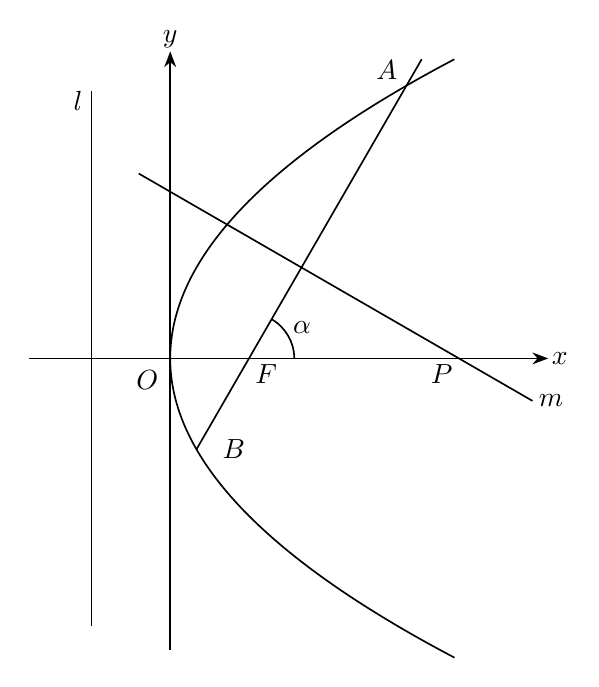
\begin{tikzpicture}[x=0.5cm,y=0.5cm,line width=.6pt,>=Stealth,font=\normalsize]
  \def\parabolaP{4}
  \def\alphaDeg{60}
  \coordinate (O) at (0,0);
  \coordinate (F) at (2,0);
  \coordinate (A) at (6,6.928203);
  \coordinate (B) at (0.666667,-2.309401);
  \coordinate (P) at (7.333333,0);
  \coordinate (mone) at (-0.8,4.695782);
  \coordinate (mtwo) at (9.2,-1.077721);
  \draw[->] (-3.6,0) -- (9.6,0) node[right,inner sep=1pt] {$x$};
  \draw[->] (0,-7.4) -- (0,7.8) node[above,inner sep=1pt] {$y$};
  \draw[domain=-7.6:7.6,samples=161,smooth,variable=\y] plot ({(\y*\y)/(2*\parabolaP)},\y);
  \draw (-2,-6.8) -- (-2,6.8);
  \draw (B) -- (6.387862,7.6);
  \draw (mone) -- (mtwo);
  \draw (F) ++(0:1.15) arc (0:\alphaDeg:1.15);
  \node[below left,inner sep=4pt] at (O) {$O$};
  \node[below right,inner sep=2pt] at (F) {$F$};
  \node at (5.5,7.32) {$A$};
  \node[right,inner sep=3pt] at (1.1,-2.3) {$B$};
  \node[below left,inner sep=2pt] at (P) {$P$};
  \node[left,inner sep=3pt] at (-2,6.55) {$l$};
  \node[right,inner sep=2pt] at (mtwo) {$m$};
  \node at (3.35,0.78) {$\alpha$};
\end{tikzpicture}
